Alex Iverson

2014-09-22

Strategizing and Brainstorming

\begin{tabular}{|p{5cm}|p{5cm}|}
 \hline
 I worked on Identifying ways to play the game.
 &
 I think we were fairly thorough. I do not anticipate seeing any major strategy elements at the tournaments we have not anticipated. I do, however, expect to encounter a combination or variation that we have not considered.
 \\
 \hline
 I helped brainstorm types of players we could build.
 &
 I would have liked to have come up with more possibilities, but I can not think of anything to add. However, it is taking a long time to analyze the ideas we have because some of the team members need to be trained how to do so; Having too many more ideas may take too much time.
 \\
 \hline
\end{tabular}

The first thing we did was try to identify what interactions with the field elements were involved in playing the game. Then we looked at how these interactions could be combined into strategies.

The first major challenge was to organize the brainstorming. Because I have more experience with designing for the FIRST competitions, I led the effort. I had difficulty conveying the distinctions between subsystems and mechanisms for the purposes of strategizing. Subsystems are categories for how the robots can interact with the field and gameplay elements, for example, a batched scorer versus a continuous feed scorer, or a rolling goal pusher versus a rolling goal grappler. They are relevant to strategy because those distinctions affect what the robots are able to do on the field. A mechanism is an implementation of a subsystem, and is largely irrelevant to strategy, because how a robot plays is much more dependent on what it can do rather than how it does it, for example, whether the robot uses a scissor lift or a forklift style pulley system to lift the balls is not important because as they are both batched scoring systems they are subject to very similar performance and limitations.

\begin{center}
 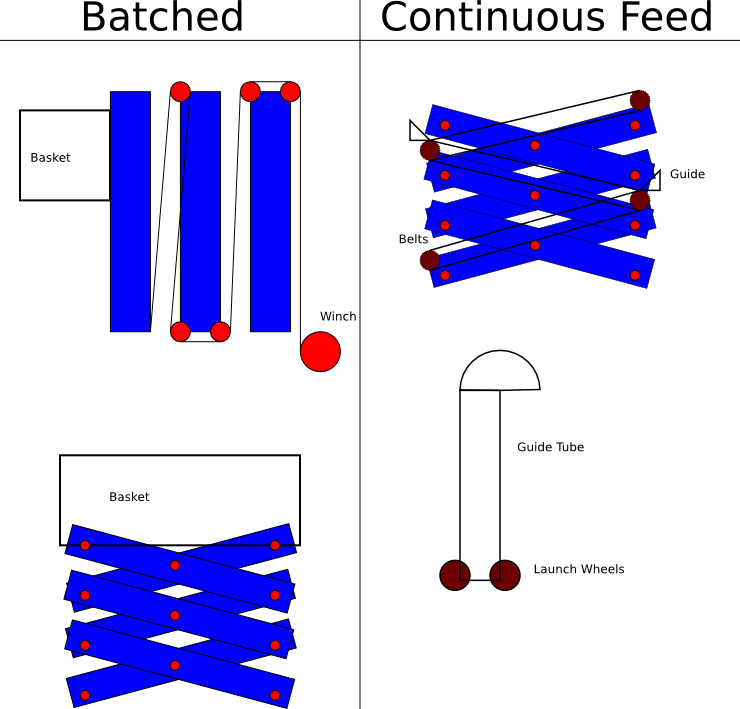
\includegraphics[width=10cm]{./Entries/Images/BatchedContinuous.png}
 % BatchedContinuous.png: 740x709 pixel, 90dpi, 20.89x20.01 cm, bb=0 0 592 567
\end{center}

We tried to estimate the performance of various subsystems to determine the effectiveness of the strategies. A batched lifter and scorer system is limited because it needs to be in a down position while collecting balls and a raised position while scoring, so its scoring rate is reduced by its travel time. A continuous feed lifter and scorer system, on the other hand is limited by needing to have a goal on hand and its requirement to handle balls in single file (this is a simplifying approximation that we assume will be proven wrong at some point.). We computed the average density of the balls based on the assumption that they would be uniformly scattered across the field area. That density allowed us to estimate the rate at which an intake of a given width would encounter balls. These calculations allowed us to estimate the scoring potentials and limiting factors of each potential design, so that we can make an informed decision about what type of robot we want to build.
